\mode*
\mode<presentation>{

  \section{Extras}
  \label{sec:extras}
  % gracias
  % preguntas
  % exp_embebidos
  % exp_biomecanica
  % exp_mecanismos
  % exp_computacion_flexible
  % exp_control
  % def_framework
  % def_problema
  % exp_capas

  \begin{frame}[label=gracias]
    \transduration{2}
    \only<1>{
      \begin{center}
        \LARGE \textbf{\textcolor{blueun}{GRACIAS POR SU ATENCI\'ON!!!}}
      \end{center}
    }
  \end{frame}
  \begin{frame}[label=preguntas]
    \only<1>{
      \begin{center}
        \LARGE \textbf{\textcolor{blueun}{Preguntas...}}
      \end{center}
    }
  \end{frame}
  % Problemas de la robotica b\'ipeda:
  % Los problemas que se intentar\'a resolver son relacionados con el uso eficiente de la energ\'ia, la din\'amica pasiva de caminadores y forman parte activa de la investigaci\'on.
  % 1) Estructuras mec\'anicas: Dise\~no de rodillas, tobillos, talon-planta-antepie, exploraci\'on de estructuras paralelas, SLIP, Curved-beams hopping robots. An\'alisis y s\'intesis para el torso.
  % 2) Capa sensora y de actuaci\'on: Reducir peso y complejidad del cableado, asegurar ancho de banda, asegurar latencias y escabilidad de la red.
  % 3) Control: Asegurar estabilidad y convergencia a los ciclos limite adem\'as auto-aprendizaje, robustez ante perturbaciones, generaci\'on On-Line, mediante Central patern generator, Redes neuronales y Logica difusa, aprendizaje de m\'aquina, LQR-Trees y Lyapunov.
  % 4) Planeaci\'on y generaci\'on de trayectorias: Optimizando la energ\'ia seg\'un el sistema mecatr\'onico proponer las trayectorias, evasi\'on de obst\'aculos. Algoritmos evolutiovos como GAs y PSOs.
  % 5) Capa de cognitiva: Agentes inteligentes, estrategias conjuntas y colaborativas.
  \begin{frame}[plain,t,label=def_problema]
    \hspace*{-0.8cm}\parbox[t]{\textwidth}{
      \only<1->{\vspace*{-0.4cm}\hspace*{-1.5cm}
        \colorbox{blueun}{
          \parbox[t][1.5cm][c]{\paperwidth}{
            \textcolor{white}{\Large\quad{PROBLEMAS DE LA ROBOTICA B\'IPEDA}}
          }
        }
      }
      \only<2-3>{\alert<2>{Los problemas que se intentar\'a resolver, comprobar o investigar son relacionados con el uso eficiente de la energ\'ia, la din\'amica pasiva de caminadores, los m\'etodos bio-inspirados y el aprendizaje de m\'aquina, adem\'as formar\'an parte activa de esta investigaci\'on.}}\\
      \only<3->{\alert<3>{Se clasifican seg\'un la capa del framework de investigaci\'on:}}
      \only<3->{\small
        \begin{columns}[t] %¡Columnas como en TeX normal!
          \begin{column}{3cm}
            \\% espacio para ajustar las graficas
            \includegraphics<5>[height=4cm]{../images/DENISE.png}
            \includegraphics<6>[height=4cm]{../images/DLR-BIPED.png}
            \includegraphics<7>[height=4cm]{../images/ASIMO.png}
            \includegraphics<8>[height=4cm]{../images/RABBIT.png}
            \includegraphics<9>[height=4cm]{../images/TODDLE-MIT.png}
          \end{column}
          \begin{column}{7cm}
            \begin{enumerate}
            \item<4-|alert@5> \hyperlink{def_problema<5>}{\textbf{Estructuras mec\'anicas\only<5>{:}} \only<5>{\scriptsize Dise\~no de rodillas, tobillos, talon-planta-antepie, exploraci\'on de estructuras paralelas, SLIP, Curved-beams hopping robots. An\'alisis y s\'intesis para el torso.}}
            \item<4-|alert@6> \hyperlink{def_problema<6>}{\textbf{Capa sensora y de actuaci\'on\only<6>{:}} \only<6>{\scriptsize Reducir peso y complejidad del cableado, asegurar ancho de banda, asegurar latencias y escabilidad de la red.}}
            \item<4-|alert@7> \hyperlink{def_problema<7>}{\textbf{Control\only<7>{:}} \only<7>{\scriptsize Asegurar estabilidad y convergencia a los ciclos limite adem\'as auto-aprendizaje, robustez ante perturbaciones, generaci\'on On-Line, mediante Central patern generator, Redes neuronales y Logica difusa, aprendizaje de m\'aquina, LQR-Trees y Lyapunov.}}
            \item<4-|alert@8> \hyperlink{def_problema<8>}{\textbf{Trayectorias\only<8>{:}} \only<8>{\scriptsize Optimizando la energ\'ia seg\'un el sistema mecatr\'onico proponer las trayectorias, evasi\'on de obst\'aculos. Algoritmos evolutiovos como GAs y PSOs.}}
            \item<4-|alert@9> \hyperlink{def_problema<9>}{\textbf{Capa de cognici\'on\only<9>{:}} \only<9>{\scriptsize Agentes inteligentes, estrategias conjuntas y colaborativas.}}
            \end{enumerate}
          \end{column}
        \end{columns}
      }\vspace{0.5cm}
      \hyperlink<4-10>{def_objetivos<3>}{\beamerreturnbutton{Volver al Objetivo General}}
    }
  \end{frame}
  \begin{frame}[plain,t,label=exp_capas]
    \transduration<1->{5}
    \hspace*{-0.8cm}\parbox[t]{\textwidth}{
      \only<1->{\vspace*{-0.4cm}\hspace*{-1.5cm}
        \colorbox{blueun}{
          \parbox[t][1.5cm][c]{\paperwidth}{
            \textcolor{white}{\Large\quad{DETALLE DE LOS OBJETIVOS GENERALES}}
          }
        }
      }\setbeamercovered{transparent}
      \only<1>{
        \begin{center}
          \parbox[c][2.0cm][c]{4cm}{}
        \end{center}
      }
      \only<2>{
        \begin{center}
          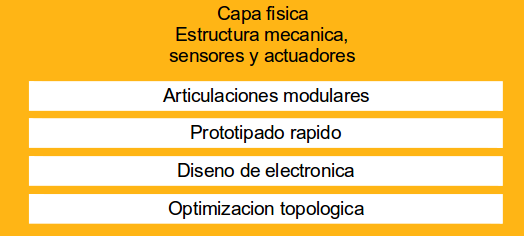
\includegraphics[height=2.0cm]{../images/objCapaFisica.png}
        \end{center}
      }
      \only<3>{
        \begin{center}
          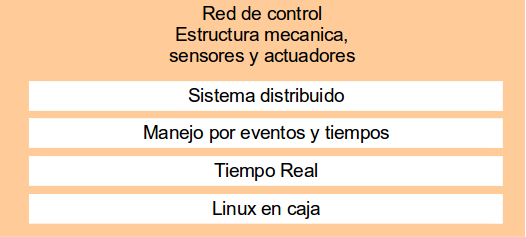
\includegraphics[height=2.0cm]{../images/objCapaRAS.png}
        \end{center}
      }
      \only<4>{
        \begin{center}
          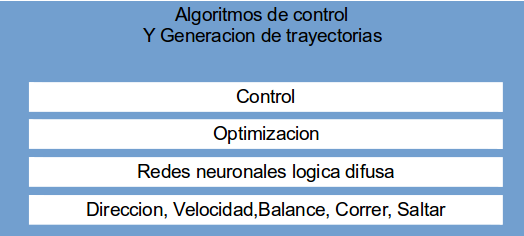
\includegraphics[height=2.0cm]{../images/objCapaControl.png}
        \end{center}
      }
      \only<5>{
        \begin{center}
          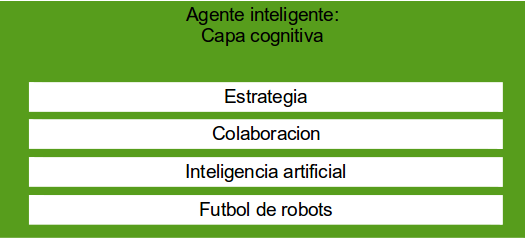
\includegraphics[height=2.0cm]{../images/objCapaCognitiva.png}
        \end{center}
      }\vspace{-0.2cm}\hspace{-1.0cm}
      \parbox[c]{12cm}{
        \begin{enumerate}[<+-|alert@+|uncover@+>][\textbf{OE:} 1.]\scriptsize
        \item Modelar, simular, analizar y sintetizar mecanismos subactuados que optimicen la energ\'ia para la locomoci\'on de caminar, saltar o correr
        \item Dise\~nar y construir una plataforma rob\'otica modular y para prototipado, capaz de configurar cadenas cinem\'aticas  controladas y/o monitoreadas bajo el sistema distribuido
        \item Implementar un sistema distribuido de sensores y actuadores que funcione en tiempo-real, bajo el principio de manejo por disparo-de-eventos y/o manejo por disparo-por-tiempos
        \item Dise\~nar, simular e implementar diferentes controles de locomoci\'on inspirados en las nuevas tendencias de investigaci\'on de caminadores sobre plataformas rob\'oticas modulares construidas
        \item Dise\~nar, simular e implementar estrategias y actividades colaborativas usando una red de caminadores
        \end{enumerate}
      }
    }
    \hyperlink{def_objesp}{\beamerreturnbutton{Volver al Objetivos Espec\'ificos}}
  \end{frame}
}